\documentclass[11pt,a4paper]{article}

\usepackage[utf8]{inputenc}
\usepackage[T1]{fontenc}
\usepackage[ngerman]{babel}
\usepackage{lmodern}
\usepackage{microtype}
\usepackage[a4paper,margin=2.15cm,headheight=15pt]{geometry}
\usepackage{amsmath}
\usepackage{booktabs}
\usepackage{tabularx}
\usepackage{array}
\usepackage{graphicx}
\usepackage{float}
\usepackage{xcolor}
\usepackage{enumitem}
\usepackage{fancyhdr}
\usepackage[hidelinks]{hyperref}
\usepackage{url}

\definecolor{projectblue}{HTML}{174A63}
\definecolor{projectteal}{HTML}{16796B}
\definecolor{lightblue}{HTML}{EAF3F6}
\definecolor{lightgray}{HTML}{F3F5F6}
\definecolor{darkgray}{HTML}{333A40}

\hypersetup{
  pdftitle={Technischer Zwischenbericht Stufe 1 - Dezentrale MRTA},
  pdfsubject={Dezentrale marktbasierte Multi-Roboter-Aufgabenzuweisung},
  pdfauthor={Projektteam},
  colorlinks=true,
  linkcolor=projectblue,
  urlcolor=projectteal
}

\pagestyle{fancy}
\fancyhf{}
\fancyhead[L]{\small Dezentrale Multi-Roboter-Aufgabenzuweisung}
\fancyhead[R]{\small Technischer Zwischenbericht - Stufe 1}
\fancyfoot[C]{\thepage}
\renewcommand{\headrulewidth}{0.4pt}

\setlength{\parindent}{0pt}
\setlength{\parskip}{0.55em}
\setlist[itemize]{leftmargin=1.5em,itemsep=0.25em,topsep=0.25em}
\setlist[enumerate]{leftmargin=1.7em,itemsep=0.25em,topsep=0.25em}
\renewcommand{\arraystretch}{1.18}

\newcommand{\statusbox}[1]{%
  \begin{center}
    \colorbox{lightblue}{\parbox{0.92\linewidth}{#1}}
  \end{center}
}

\newcommand{\codepath}[1]{\texttt{\detokenize{#1}}}

\begin{document}

\hypersetup{pageanchor=false}
\begin{titlepage}
  \thispagestyle{empty}
  \vspace*{1.4cm}
  {\color{projectteal}\rule{\textwidth}{3pt}}

  \vspace{1.2cm}
  {\Huge\bfseries\color{projectblue}
    Dezentrale marktbasierte\\[0.25em]
    Multi-Roboter-Aufgabenzuweisung\par}

  \vspace{0.7cm}
  {\LARGE Technischer Zwischenbericht - Stufe 1\par}

  \vspace{0.45cm}
  {\large Tier-0-Simulation, Bidding-Protokoll und empirischer Baseline-Vergleich\par}

  \vfill

  \statusbox{
    \textbf{Dokumentstatus:} Arbeitsfähige Basis für die nächste Projektstufe.\\[0.35em]
    \textbf{Kernstand:} Dezentrale Auktion implementiert, Simulation und Replays verfügbar,
    Parametersuche und getrennte Holdout-Auswertung abgeschlossen, 18 Tests erfolgreich.
  }

  \vfill
  \begin{tabular}{@{}ll@{}}
    Projektphase: & Stufe 1 / Tier 0\\
    Dokumenttyp: & Technische Zusammenfassung und Übergabebasis\\
    Stand: & 11. August 2026\\
    Implementierung: & Python 3.11 oder neuer
  \end{tabular}

  \vspace{1.2cm}
  {\color{projectteal}\rule{\textwidth}{3pt}}
\end{titlepage}

\hypersetup{pageanchor=true}
\pagenumbering{roman}
\begingroup
\small
\setlength{\parskip}{0pt}
\tableofcontents
\endgroup
\clearpage
\pagenumbering{arabic}

\section{Kurzfassung}

Die erste Projektstufe ist als lauffähiger, reproduzierbarer Prototyp umgesetzt. Die
Roboter verteilen Aufgaben über ein dezentrales Peer-to-Peer-Auktionsverfahren. Ein
Roboter entdeckt oder erzeugt eine Aufgabe, kündigt sie mit \texttt{ANNOUNCE} an,
erhält lokale Gebote über \texttt{BID} und vergibt sie mit \texttt{AWARD}. Es existiert
kein zentraler Allocator, der globale Zustände sammelt oder Gewinner auswählt.

Die Logik wird in einer schnellen zweidimensionalen Tier-0-Simulation in einer
$2\,\mathrm{m}\times2\,\mathrm{m}$-Arena geprüft. Simuliert werden sieben Roboter,
Bewegung, Startverzögerung, Akkuverbrauch, Funklatenzen, Paketverlust, Erkennung und die
Aufgabentypen \texttt{GUARD}, \texttt{PUSH}, \texttt{SURROUND} und \texttt{SURVEY}.

Die Marktstrategie wird unter identischen physischen und stochastischen Bedingungen mit
Nearest Greedy, Random Assignment und einer Greedy-Ablation ohne \texttt{SURVEY}
verglichen. Auf 40 getrennten Holdout-Seeds erreicht Market einen
operationalen Score von \textbf{0,861}, gegenüber \textbf{0,831} bei Nearest Greedy und
\textbf{0,813} bei Random Assignment. Gegen Nearest Greedy ist Market im Mittel rund
\textbf{10,08 Sekunden schneller} und verteilt die Arbeitslast gleichmäßiger.

Zur qualitativen Prüfung existiert ein interaktiver 2D-Replay-Player mit Start/Pause,
Zeitleiste, Einzelschritten, einstellbarer Geschwindigkeit, Fahrspuren und sichtbaren
Robotern sowie Aufgaben. Die vollständigen Logs, statistischen Ergebnisse, Diagramme,
Parameter und 18 automatischen Tests sind Teil des Projektordners.

\statusbox{
  \textbf{Zentrale Aussage:} Für die dokumentierte Tier-0-Szenariofamilie liefert die
  dezentrale Marktstrategie einen statistisch abgesicherten höheren operationalen
  Gesamtscore als Nearest Greedy und Random Assignment. Dies ist ein reproduzierbarer
  empirischer Nachweis, aber noch kein universeller mathematischer Dominanzbeweis und
  noch kein Nachweis für Webots oder reale Pi-Pucks.
}

\section{Zielsetzung und Abgrenzung}

Ziel der ersten Stufe ist eine belastbare Software- und Versuchsbasis für dezentrale
Multi-Roboter-Aufgabenzuweisung (MRTA). Dazu gehören:

\begin{itemize}
  \item eine plattformunabhängige, dezentrale Zuweisungslogik,
  \item ein schnelles Simulationsmodell für viele reproduzierbare Versuche,
  \item faire Baselines mit identischen Szenarien und Zufallsseeds,
  \item eine nachvollziehbare Parameterwahl ohne Vermischung von Training und Nachweis,
  \item portable Logs, statistische Auswertung und visuelle Replays,
  \item eine klar definierte Schnittstelle für Webots und reale Pi-Puck-Roboter.
\end{itemize}

Die aktuelle Stufe modelliert Roboter als Punktroboter in einer ebenen Arena. Sie ist
bewusst schneller und einfacher als eine physiknahe Webots-Simulation. Reale
Differentialantriebsdynamik, Sensorrauschen, Kollisionen, Lokalisierungsfehler und echte
Netzwerkeffekte müssen in der nächsten Stufe kalibriert beziehungsweise ergänzt werden.

\section{Systemarchitektur}

\subsection{Schichten und Portabilität}

Die Architektur trennt die eigentliche Allokationsentscheidung von Simulation,
Hardware und Auswertung:

\begin{center}
\setlength{\fboxsep}{8pt}
\fbox{\parbox{0.82\linewidth}{
  \centering
  \textbf{experiments/}\\
  Läufe, Parametersuche, Statistik, Plots und Replays\\[0.55em]
  $\downarrow$\\[0.35em]
  \textbf{sim/ und backends/}\\
  Tier-0-Welt oder später Webots-/Pi-Puck-Adapter\\[0.55em]
  $\downarrow$\\[0.35em]
  \textbf{allocation/}\\
  Plattformunabhängige Tasks, Gebote, Nachrichten und Auktionen
}}
\end{center}

Das Paket \codepath{allocation/} verwendet nur die Python-Standardbibliothek und
importiert weder Simulation noch Metriken. Die physische Plattform wird über acht kleine
Backend-Fähigkeiten angebunden: Pose lesen, Akku lesen, Ziel anfahren, Zielerreichung
prüfen, Nachricht senden, Nachrichten empfangen, RoIs erkennen und Zeit lesen. Dadurch
sollen Webots und Pi-Pucks später dieselbe Allokationslogik unverändert nutzen.

\subsection{Dezentraler Auktionsablauf}

\begin{enumerate}
  \item Ein Roboter erkennt eine Region of Interest (RoI) oder erzeugt eine fällige
        \texttt{SURVEY}-Aufgabe und wird für genau diese Aufgabe Auctioneer.
  \item Er sendet \texttt{ANNOUNCE} mit Aufgabenart, Position, benötigter Teamgröße,
        Prioritätsfunktion und Gebotsdeadline.
  \item Jeder erreichbare Roboter berechnet ein Gebot ausschließlich aus seinem lokalen
        Zustand und sendet \texttt{BID}.
  \item Der lokale Auctioneer sortiert die Paare aus Kosten und Roboter-ID und sendet
        \texttt{AWARD} an die günstigsten $n_{req}$ Roboter.
  \item Die Gewinner navigieren zum Ziel. Eine Mehrroboteraufgabe startet erst, wenn die
        exakt benötigte Zahl an Gewinnern angekommen ist.
  \item Abschluss und Rückgabe werden über \texttt{DONE} oder \texttt{RELEASE}
        verbreitet. Bei einer Rückgabe kann der ursprüngliche Auctioneer erneut bieten
        lassen.
\end{enumerate}

Die fünf Nachrichtentypen \texttt{ANNOUNCE}, \texttt{BID}, \texttt{AWARD},
\texttt{DONE} und \texttt{RELEASE} sind kompakt und deterministisch als JSON-Bytes
serialisiert. Funklatenz und Paketverlust werden unabhängig pro Empfänger simuliert.

\subsection{Warum kein zentraler Allocator vorliegt}

Jede Roboterinstanz führt ihren lokalen Aufgabenbestand, lokale Gebote, laufende
Aufträge und selbst gehostete Auktionen. Die Welt erzeugt Ereignisse und simuliert
Bewegung, Funk sowie physische Ausführung, wählt aber keine Auktionsgewinner. Es gibt
somit keine globale Instanz, die alle Roboterzustände für eine zentrale Entscheidung
zusammenführt.

\section{Bidding, Priorität und Preemption}

\subsection{Gebotskosten}

Das niedrigste Gebot gewinnt. Die drei Kostenterme sind auf $[0,1]$ normiert:

\begin{equation}
  c_i(\mathrm{task}) = \alpha\,\hat d_i + \beta\,\hat w_i
  + \gamma\,(1-\hat e_i).
\end{equation}

Dabei bezeichnet $\hat d_i$ die geschätzte Distanz, $\hat w_i$ die aktuelle Last und
$\hat e_i$ die verbleibende Energie von Roboter $i$. Die Priorität steht nicht direkt im
Gebot, weil sie innerhalb einer einzelnen Auktion alle Gebote nur um dieselbe Konstante
verschieben würde. Stattdessen steuert sie den Wettbewerb zwischen bereits laufenden und
neu eintreffenden Aufgaben.

\subsection{Zeitabhängige Priorität}

Die Priorität altert nach

\begin{equation}
  p(\Delta t)=p_0+(1-p_0)\left(1-\exp\left[-(\lambda\Delta t)^k\right]\right).
\end{equation}

Eine Preemption ist nur während \texttt{NAVIGATE}, niemals während
\texttt{WAIT\_PEERS} oder \texttt{EXECUTE}, zulässig. Sie wird ausgelöst, wenn

\begin{equation}
  \delta\,(p_{new}-p_{current})-(c_{new}-c_{current})>\theta_{hyst}.
\end{equation}

Zusätzlich begrenzt ein Cooldown von 15 Sekunden unnötiges Wechseln. Dadurch bleiben
bereits synchronisierte oder ausgeführte Teamaufgaben stabil.

\subsection{Gewählte Parameter}

\begin{table}[H]
\centering
\begin{tabularx}{0.88\textwidth}{@{}l r X@{}}
\toprule
Parameter & Wert & Bedeutung\\
\midrule
$\alpha$ & 1,0 & Gewicht der normalisierten Distanz\\
$\beta$ & 0,5 & Gewicht der aktuellen Arbeitslast\\
$\gamma$ & 0,0 & Gewicht der Batteriereserve im 300-Sekunden-Hauptszenario\\
$\delta$ & 1,5 & Einfluss des Prioritätsgewinns bei Preemption\\
$\theta_{hyst}$ & 0,1 & Hysterese gegen unnötige Auftragswechsel\\
\bottomrule
\end{tabularx}
\caption{Durch die Trainingssuche gewählte Market-Parameter.}
\end{table}

Der Wert $\gamma=0$ ist ein Ergebnis der Suche und kein ausgelassener Term. Im
300-Sekunden-Holdout wird kein Roboter vollständig entladen. Ein stärkerer Batterieterm
erzeugt dort zusätzliche Wege, ohne einen Ausfall zu verhindern. Für längere Einsätze
bleibt $\gamma$ im Suchraum und das Batteriemodell ist implementiert.

\section{Tier-0-Simulation}

\subsection{Hauptkonfiguration}

\begin{table}[H]
\centering
\small
\begin{tabularx}{\textwidth}{@{}l l X@{}}
\toprule
Bereich & Standardwert & Modellierung\\
\midrule
Arena & $2\,\mathrm{m}\times2\,\mathrm{m}$ & zweidimensionale Punktroboterwelt\\
Roboter & 7 & heterogene Startposition und zufälliger Startakku\\
Laufzeit & 300 s bei $\Delta t=0{,}1$ s & schnelle deterministische Zeitschritte\\
Bewegung & 0,08 m/s & effektive Geschwindigkeit plus 1,2 s Startverzögerung\\
Ereignisse & 28 RoIs & feste Hotspots, für alle Strategien identisch\\
Erkennung & Radius 0,30 m & RoI wird bei räumlicher Nähe erkannt\\
Funk & 5--40 ms, 2\,\% Verlust & unabhängige Zustellung pro Empfänger\\
Akku & 0,26--1,00 initial & Idle- und wegabhängige Entladung, Depletion-Schwelle 0,05\\
Coverage & 0,05-m-Zellen & SURVEY-Zellen von 0,4 m und zeitabhängige Idleness\\
\bottomrule
\end{tabularx}
\caption{Zentrale Standardwerte aus \codepath{parameters/default.json}.}
\end{table}

\subsection{Aufgabentypen}

\begin{table}[H]
\centering
\begin{tabularx}{0.92\textwidth}{@{}l c c X@{}}
\toprule
Typ & Roboter & Dauer & Rolle im Szenario\\
\midrule
\texttt{GUARD} & 1 & 15 s & Einzelroboter sichert eine erkannte RoI\\
\texttt{PUSH} & 2 & 20 s & koordinierte Zwei-Roboter-Aufgabe\\
\texttt{SURROUND} & 3 & 10 s & koordinierte Drei-Roboter-Aufgabe\\
\texttt{SURVEY} & 1 & variabel & räumliche Abdeckung und erneute Erkundung alter Zellen\\
\bottomrule
\end{tabularx}
\caption{Unterstützte Aufgabentypen und Teamgrößen.}
\end{table}

\texttt{SURVEY} zählt nicht zur normalen Arbeitslast und kann für eine neu erkannte RoI
ohne Hysterese freigegeben werden. Mehrroboteraufgaben werden erst physisch ausgeführt,
wenn alle benötigten Gewinner am Ziel sind.

\section{Baselines und fairer Vergleich}

Vier Strategien laufen in derselben Simulations- und Kommunikationsinfrastruktur:

\begin{itemize}
  \item \textbf{Market:} dezentrale Kosten aus Distanz, Last und optional Batterie.
  \item \textbf{Nearest Greedy:} bevorzugt den lokal nächstgelegenen geeigneten Roboter.
  \item \textbf{Random Assignment:} weist unter geeigneten Robotern zufällig zu.
  \item \textbf{Nearest Greedy ohne SURVEY:} Ablation zur getrennten Bewertung des
        Erkundungsverhaltens und seiner Kommunikationskosten.
\end{itemize}

Szenario, Funk und Random-Baseline besitzen getrennte, aus dem Lauf-Seed abgeleitete
Zufallsgeneratoren. Derselbe Seed erzeugt damit für alle Strategien dasselbe physische
Szenario. Ein identischer Lauf ist deterministisch und erzeugt byte-identische
Ereignislogs. Die Strategien unterscheiden sich in der Zuweisungsentscheidung, nicht in
der zugrunde liegenden Welt.

\section{Parametersuche und Nachweismethodik}

\subsection{Trennung von Auswahl und Auswertung}

Die Konfiguration wurde ausschließlich auf den Trainings-Seeds 0 bis 7 ausgewählt. Der
anschließende Nachweis verwendet die davon getrennten 40 Holdout-Seeds 1000 bis 1039.
Jeder Holdout-Seed wird mit allen vier Strategien gerechnet. So kann pro Seed eine
gerichtete gepaarte Differenz gebildet werden, ohne dass unterschiedliche Zufallsfälle
den Strategievergleich verzerren.

Die Gittersuche variiert $\beta$, $\gamma$, $\delta$ und $\theta_{hyst}$. Aus 14
nicht-dominierten Pareto-Punkten wird der Punkt mit dem höchsten vorab dokumentierten
operationalen Score gewählt.

\subsection{Operationaler Score}

\begin{table}[H]
\centering
\small
\begin{tabular}{@{}lr@{\qquad}lr@{}}
\toprule
Komponente & Gewicht & Komponente & Gewicht\\
\midrule
Completion Rate & 0,30 & Detection Rate & 0,10\\
Bearbeitungszeit & 0,10 & Lastbalance & 0,15\\
Coverage & 0,05 & mittlere Idleness & 0,08\\
Detektionslatenz & 0,07 & Restakku & 0,05\\
keine Depletion & 0,10 & & \\
\bottomrule
\end{tabular}
\caption{Vorab dokumentierte Gewichte des operationalen Scores.}
\end{table}

Alle Komponenten werden vor der Gewichtung auf $[0,1]$ begrenzt. Der Score dient der
Gesamtbewertung und Parameterwahl, ersetzt aber nicht die einzeln berichteten Metriken.

\subsection{Statistik}

Für jede Baseline werden Mittelwert der gepaarten Differenzen, ein nichtparametrisches
95\,\%-Bootstrap-Konfidenzintervall mit 20.000 Resamples, ein gepaarter
Vorzeichen-Randomisierungstest mit 20.000 Ziehungen, die Win-Rate über 40 Seeds und
Holm-korrigierte p-Werte berichtet. Ein Vorteil wird nur dann als solcher bezeichnet,
wenn das Konfidenzintervall vollständig positiv ist und $p_{Holm}<0{,}05$ gilt.

\section{Ergebnisse}

\subsection{Holdout-Mittelwerte}

\begin{table}[H]
\centering
\small
\begin{tabular}{@{}lrrrrrr@{}}
\toprule
Strategie & Score & Completion & Zeit [s] & Load-SD & Max. Idle [s] & Msg/Task\\
\midrule
Market & \textbf{0,861} & \textbf{0,918} & \textbf{37,76} & \textbf{1,42} & 264,99 & 40,26\\
Nearest Greedy & 0,831 & 0,887 & 47,84 & 1,84 & 267,09 & 38,28\\
Greedy ohne SURVEY & 0,813 & 0,861 & 46,98 & 2,09 & 238,70 & 10,70\\
Random Assignment & 0,813 & 0,788 & 59,60 & 1,35 & 284,29 & 43,72\\
\bottomrule
\end{tabular}
\caption{Mittelwerte auf den 40 Holdout-Seeds. Kleinere Zeiten, Load-SD und Idleness
sind besser; höhere Scores und Completion Rates sind besser.}
\end{table}

\subsection{Wichtigste gepaarte Effekte}

Gegen Nearest Greedy beträgt der Score-Vorteil von Market $+0{,}0305$ mit einem
95\,\%-Bootstrap-Konfidenzintervall von $[+0{,}0151;+0{,}0462]$, einer Win-Rate von
77,5\,\% und $p_{Holm}=0{,}0040$. Die mittlere Bearbeitungszeit verbessert sich um
10,08 Sekunden; das Intervall $[6{,}46;13{,}72]$ liegt vollständig über null und die
Win-Rate beträgt 87,5\,\%. Die Laststreuung sinkt um 0,42 Aufgaben.

Gegen Random Assignment steigt der Score im Mittel um 0,0479 und die Completion Rate
um 0,1295. Die Bearbeitungszeit verbessert sich um 21,85 Sekunden. Alle drei Effekte
sind im gepaarten Holdout signifikant. Damit zeigt die Marktstrategie besonders bei
koordinierter Erledigung und zeitlicher Effizienz einen klaren Vorteil.

\begin{figure}[H]
  \centering
  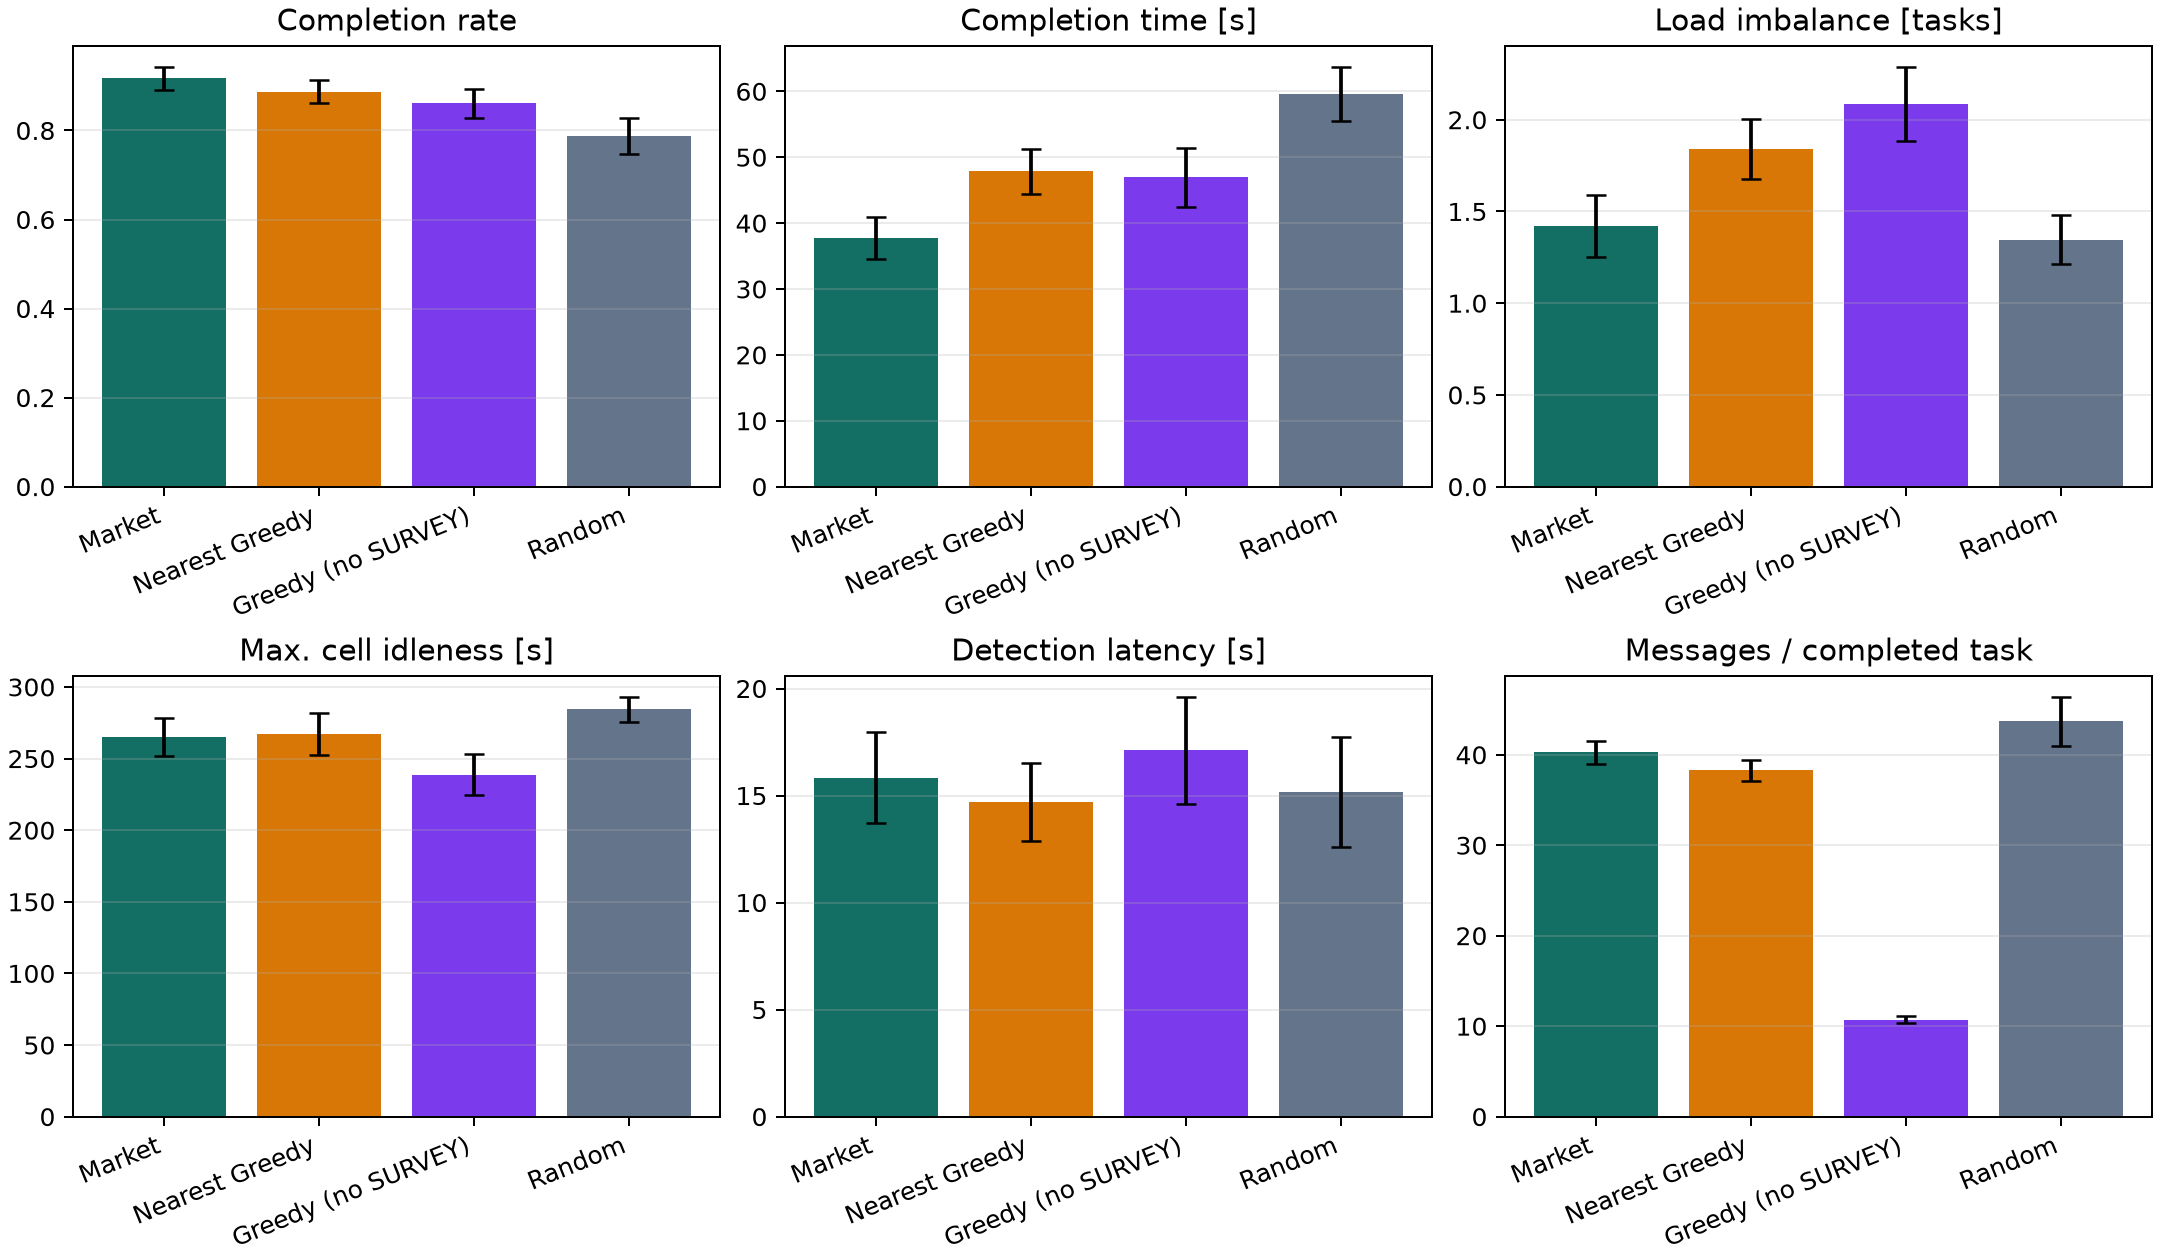
\includegraphics[width=\textwidth]{results/comparison.png}
  \caption{Ausgewählte Holdout-Metriken. Die Fehlerbalken zeigen die Streuung der
  Strategieergebnisse über die ausgewerteten Szenarien.}
\end{figure}

\subsection{Trade-offs und korrekte Interpretation}

Market gewinnt nicht zwangsläufig jede Einzelmetrik. Gegen Nearest Greedy werden im
Mittel rund zwei zusätzliche Nachrichten pro abgeschlossener Aufgabe benötigt; nach
Mehrfachkorrektur ist dieser Unterschied knapp nicht signifikant. Der mittlere Restakku
ist geringfügig niedriger. Random Assignment kann zufällig eine sehr gleichmäßige Last
erzeugen, erledigt aber deutlich weniger Aufgaben und benötigt länger.

Greedy ohne \texttt{SURVEY} erzeugt erwartungsgemäß wesentlich weniger Nachrichten und
hat in diesem Boustrophedon-Szenario eine geringere maximale Idleness. Dafür verliert die
Ablation bei Completion, Bearbeitungszeit und Lastbalance. Diese Preise werden offen
berichtet und nicht durch den Gesamtscore verdeckt.

\begin{figure}[H]
  \centering
  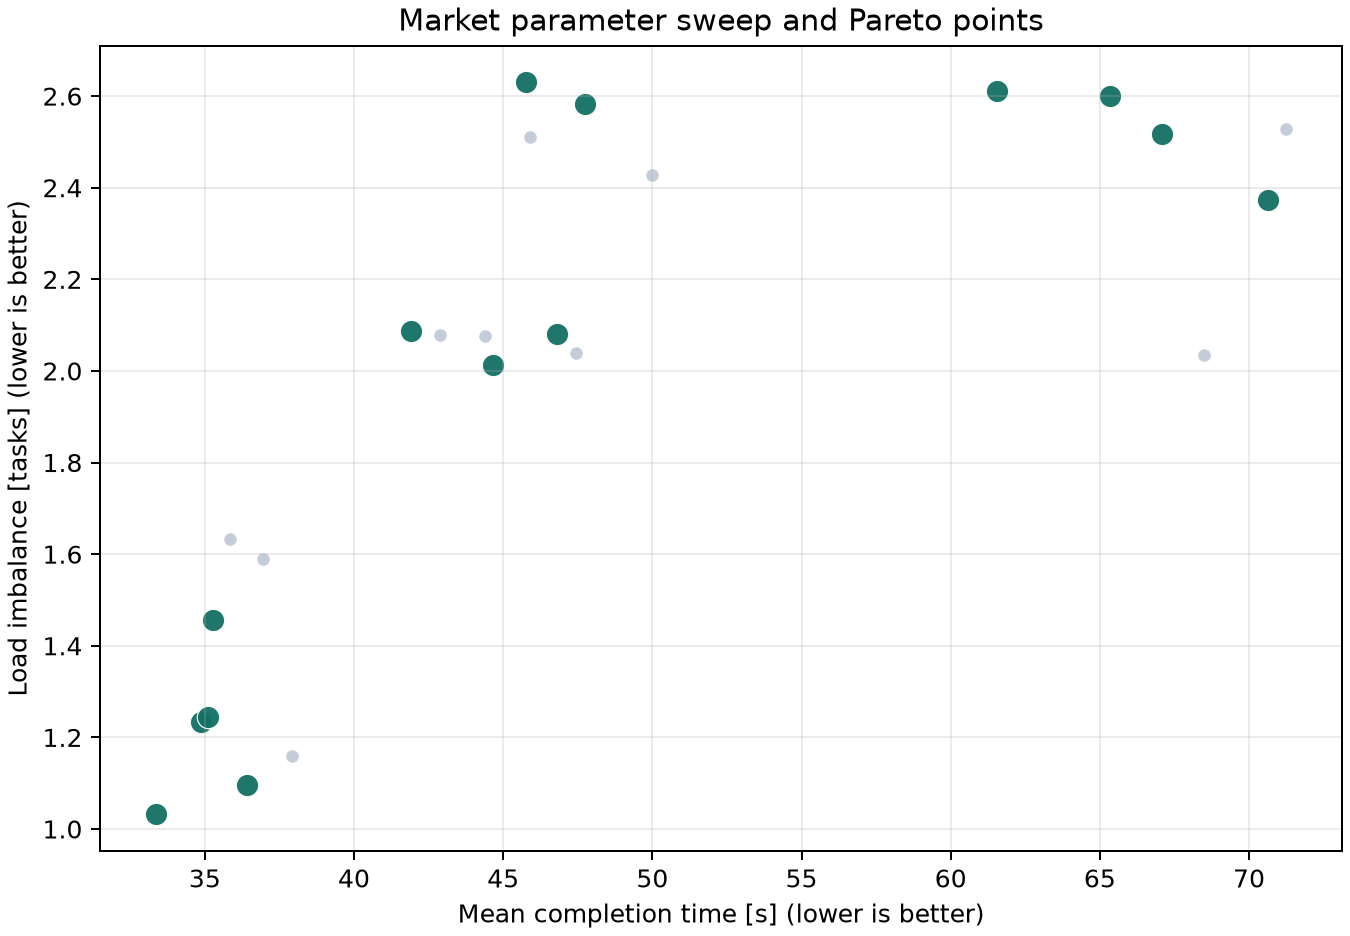
\includegraphics[width=0.92\textwidth]{results/pareto.png}
  \caption{Parametersuche: mittlere Bearbeitungszeit gegen Lastungleichgewicht. Dunkle
  Punkte markieren nicht-dominierte Parameterkonfigurationen.}
\end{figure}

\section{Logging, Replays und Tests}

Jeder Lauf schreibt portable Dateien in den gewählten Logordner:

\begin{itemize}
  \item \codepath{events.csv}: Auktionen, Gebote, Zuweisungen, Ausführung und Abschluss,
  \item \codepath{state.csv}: Position und Zustand der Roboter über die Zeit,
  \item \codepath{metadata.json}: Seed, Strategie, Parameter und Laufkonfiguration,
  \item \codepath{replay.html}: interaktiver Offline-Player,
  \item optional \codepath{replay.gif}: nicht interaktive Animation.
\end{itemize}

Der HTML-Player zeigt die Roboterbewegung in der 2D-Arena sowie Aufgaben und
Zuweisungen. Play/Pause, Zeitregler, Schritte von einer Sekunde, Geschwindigkeiten von
0,25-fach bis 20-fach, Fahrspuren, SURVEY-Ebenen, Leertaste und Pfeiltasten erlauben eine
gezielte visuelle Analyse. Er läuft lokal im Browser ohne Server und ohne
Internetverbindung.

Die Testsuite enthält 18 Unit- und Invariantentests. Sie prüft unter anderem
Nachrichtenformate, Gebots- und Auktionslogik, Priorität, Determinismus,
Mehrroboter-Synchronisation, Depletion und \texttt{RELEASE}, Paketverlust,
plattformunabhängige Imports und die Integrität der Simulationsabläufe.

\section{Bedienung und Reproduktion}

Der Projektordner kann auf einem beliebigen Computerpfad entpackt werden. Es existiert
keine Abhängigkeit von einem persönlichen Windows-Benutzernamen. Benötigt wird Python
3.11 oder neuer. Alle Befehle werden im Ordner ausgeführt, in dem \codepath{README.md}
und \codepath{pyproject.toml} liegen.

\subsection{Installation und Tests}

\begin{verbatim}
python -m pip install -e .
python -m unittest discover -s tests -v
\end{verbatim}

\subsection{Empfohlener Lauf mit interaktivem Replay}

\begin{verbatim}
python -m experiments.run_once --strategy market --seed 42 \
  --output logs\market_42 --interactive-replay
\end{verbatim}

Danach wird \codepath{logs/market_42/replay.html} im Browser geöffnet. Für einen fairen
visuellen Vergleich werden derselbe Seed und getrennte Ausgabeordner verwendet, während
\texttt{market} nacheinander durch \texttt{nearest\_greedy} und
\texttt{random\_assignment} ersetzt wird.

\subsection{Vollständige Auswertung}

\begin{verbatim}
python -m experiments.compare
\end{verbatim}

Der Befehl reproduziert Parametersuche, Holdout-Läufe, Statistik und Abbildungen. Auf der
Entwicklungsmaschine benötigt er ungefähr 2,5 Minuten; die Laufzeit kann auf anderen
Computern abweichen. Die bereits berechneten Resultate liegen im Ordner
\codepath{results/} und müssen zum Lesen oder Präsentieren nicht neu erzeugt werden.

\section{Grenzen des aktuellen Nachweises}

Die Ergebnisse gelten für die implementierte Tier-0-Szenariofamilie, die dokumentierten
Parameter und die 40 Holdout-Seeds. Sie belegen keine universelle Überlegenheit der
Marktstrategie und garantieren nicht, dass dieselbe Rangfolge in Webots oder auf realen
Robotern bestehen bleibt.

Insbesondere müssen folgende Punkte in späteren Stufen berücksichtigt werden:

\begin{itemize}
  \item reale Kinematik, Beschleunigung, Drehzeiten und Kollisionsvermeidung,
  \item Sensorrauschen, Sichtfeld, Fehl- und Mehrfachdetektionen,
  \item Lokalisierungsfehler und Koordinatentransformationen,
  \item Reichweite, Verzögerung, Burst-Verluste und Duplikate echter Funknetze,
  \item reale Akkuentladung unter Fahrt, Stillstand, Sensorik und Kommunikation,
  \item Roboterausfälle, blockierte Wege und Recovery-Strategien,
  \item Skalierung auf andere Arena-, Team- und Aufgabengrößen.
\end{itemize}

\section{Empfohlener nächster Schritt: Webots und Pi-Pucks}

Die nächste Stufe sollte die bestehende Allokationslogik nicht neu schreiben, sondern
die acht Backend-Fähigkeiten für Webots und anschließend für Pi-Pucks implementieren.
Ein sinnvoller Übergang besteht aus vier Schritten:

\begin{enumerate}
  \item \textbf{Schnittstellen einfrieren:} Nachrichtenformat, Koordinatensystem,
        Zeiteinheit, Robot-IDs, Fehlerzustände und Semantik der acht Backend-Funktionen
        gemeinsam abstimmen.
  \item \textbf{Webots-Adapter bauen:} Pose, Batterie, Bewegung, Zielerreichung,
        Kommunikation, Detektion und Uhrzeit an die vorhandene Schnittstelle anbinden.
  \item \textbf{Tier 1 kalibrieren:} Insbesondere \texttt{effective\_speed},
        \texttt{startup\_delay}, Ankunftstoleranz, Funkverlust, Latenz und Batteriemodell
        durch Messläufe an Webots beziehungsweise Pi-Pucks bestimmen.
  \item \textbf{Gepaarten Vergleich wiederholen:} Market, Nearest Greedy und Random mit
        identischen Webots-Seeds und danach identischen Realversuchen vergleichen. Die
        Tier-0-Analyse dient dabei als Referenz, nicht als vorausgesetztes Ergebnis.
\end{enumerate}

Als unmittelbare Teamentscheidung sollten zunächst die Zielplattform, verfügbare
Pi-Puck-Hardware, Webots-Version, Kommunikationsart, RoI-Sensorik und das gemeinsame
Koordinatensystem festgelegt werden. Danach kann der Backend-Adapter implementiert und
gegen die vorhandenen 18 Tests sowie neue Hardware-in-the-Loop-Tests geprüft werden.

\section{Projektartefakte}

\begin{tabularx}{\textwidth}{@{}l X@{}}
\toprule
Pfad & Inhalt\\
\midrule
\codepath{allocation/} & Plattformunabhängige Tasks, Gebote, Nachrichten und Auktionen\\
\codepath{backends/} & Acht-Fähigkeiten-Schnittstelle und Tier-0-Adapter\\
\codepath{sim/} & Roboter, Arena, Funk, Batterie, Coverage und Ereignisse\\
\codepath{metrics/} & CSV-Logging und Metrikberechnung\\
\codepath{experiments/} & Läufe, Parametersuche, Statistik, Plots und Replays\\
\codepath{parameters/} & Standardparameter und Suchraum\\
\codepath{tests/} & 18 automatisierte Unit- und Invariantentests\\
\codepath{logs/example/} & Fertiger Beispiel-Log mit GIF und interaktivem HTML-Replay\\
\codepath{results/} & Vollständige Holdout-Ergebnisse, Tabellen und Abbildungen\\
\codepath{docs/} & Architektur, Methodik und Anforderungszuordnung\\
\codepath{references/} & Ursprüngliches Briefing und Projektvorschlag als PDF\\
\bottomrule
\end{tabularx}

\section{Fazit}

Stufe 1 liefert eine funktionsfähige, dezentrale MRTA-Basis mit klarer
Plattformtrennung, reproduzierbarer Simulation, fairen Baselines, statistisch getrenntem
Training und Holdout sowie visueller und maschinenlesbarer Nachvollziehbarkeit. Der
Marktansatz verbessert in der untersuchten Szenariofamilie den operationalen Score, die
Bearbeitungszeit und gegenüber Nearest Greedy auch die Lastverteilung.

Damit ist die Grundlage für den nächsten Schritt vorhanden: die bestehende Logik über
einen Webots- und später Pi-Puck-Backend-Adapter auf realistischere Dynamik zu übertragen,
Parameter messtechnisch zu kalibrieren und denselben gepaarten Vergleich auf Tier 1 und
Hardware zu wiederholen.

\vfill
\begin{center}
\small\color{darkgray}
Maßgebliche maschinenlesbare Konfiguration: \codepath{parameters/default.json}.\\
Vollständige Auswertung: \codepath{results/comparison_summary.md} und
\codepath{results/paired_effects.csv}.
\end{center}

\end{document}
